\clearpage
\section{\RU{Множество Мандельброта}\EN{Mandelbrot set}}
\label{Mandelbrot_demo}

\RU{Я нашел дему}\EN{Just found a demo}\footnote{Download it \href{http://go.yurichev.com/17306}
{\RU{здесь}\EN{here}},} 
\RU{написанную автором по имени}\EN{written by} ``Sir\_Lagsalot'' \InENRU 2009, 
\RU{рисующая множество Мандельброта, и это программа для x86 с размером файла всего 64 байта}\EN{drawing 
Mandelbrot set which is just a x86 program with executable 
file size only 64 bytes}.
\RU{Там только 30 16-битных x86-инструкций}\EN{There are only 30 16-bit x86 instructions}.

\RU{Вот что она рисует}\EN{Here it is what it draws}:

\begin{figure}[H]
\centering
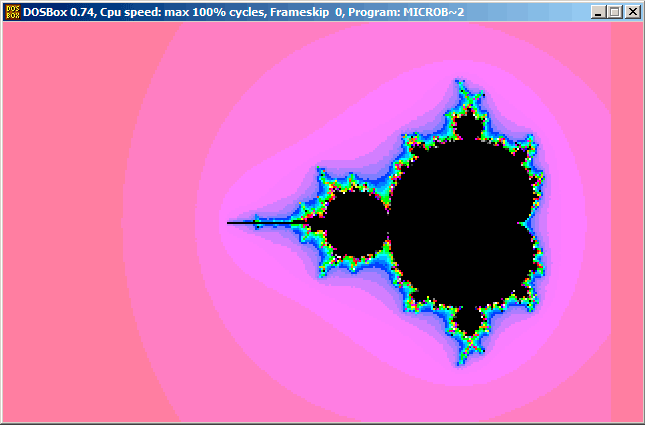
\includegraphics[scale=\FigScale]{examples/demos/mandelbrot/1.png}
\end{figure}

\RU{Попробуем разобраться, как она работает}\EN{Let's try to understand, how it works}.

\clearpage
\subsection{\RU{Теория}\EN{Theory}}

\subsubsection{\RU{Немного о комплексных числах}\EN{A word about complex numbers}}

\RU{Комплексное число состоит из двух чисел (вещественная (Re) и мнимая (Im).}
\EN{Complex number is a number consisting of two (real (Re) and imaginary (Im) parts).}

\RU{Комплексная плоскость --- это двухмерная плоскость, где любое комплексное число может быть расположено:
вещественная часть --- это одна координата и мнимая --- вторая.}
\EN{Complex plane is a two-dimensional plane where any complex number can be placed: real part is one coordinate
and imaginary part is another.}

\RU{Некоторые базовые правила, которые нам понадобятся}\EN{Some basic rules we need to know}:

\begin{itemize}
\item \RU{Сложение}\EN{Addition}: $(a+bi) + (c+di) = (a+c) + (b+d)i$

\RU{Другими словами}\EN{In other words}:

$\operatorname{Re}(sum) = \operatorname{Re}(a) + \operatorname{Re}(b)$

$\operatorname{Im}(sum) = \operatorname{Im}(a) + \operatorname{Im}(b)$

\item \RU{Умножение}\EN{Multiplication}: $(a+bi) (c+di) = (ac-bd) + (bc+ad)i$

\RU{Другими словами}\EN{In other words}:

$\operatorname{Re}(product) = \operatorname{Re}(a) \cdot \operatorname{Re}(c) - \operatorname{Re}(b) \cdot \operatorname{Re}(d)$

$\operatorname{Im}(product) = \operatorname{Im}(b) \cdot \operatorname{Im}(c) + \operatorname{Im}(a) \cdot \operatorname{Im}(d)$

\item \RU{Возведение в квадрат}\EN{Square}: $(a+bi)^2 = (a+bi) (a+bi) = (a^2-b^2) + (2ab)i$

\RU{Другими словами}\EN{In other words}:

$\operatorname{Re}(square) = \operatorname{Re}(a)^2-\operatorname{Im}(a)^2$

$\operatorname{Im}(square) = 2 \cdot \operatorname{Re}(a) \cdot \operatorname{Im}(a)$

\end{itemize}

\subsubsection{\RU{Как нарисовать множество Мандельброта}\EN{How to draw Mandelbrot set}}

\RU{Множество Мандельброта --- это набор точек, для которых рекурсивное соотношение}
\EN{Mandelbrot set is a set of points for which} $z_{n+1} = {z_n}^2 + c$ 
(\RU{где}\EN{where} $z$ \AndENRU $c$ \RU{это комплексные числа и}\EN{are complex numbers and} $c$ 
\RU{это начальное значение}\EN{is starting value})
\RU{не стремится к бесконечности}\EN{recursive sequence is not approach infinity}.\\
\\
\RU{Простым русским языком}\EN{In plain English language}: 

\begin{itemize}
\item \RU{Перечисляем все точки на экране}\EN{Enumerate all points on screen}. 
\item \RU{Проверяем, является ли эта точка в множестве Мандельброта}\EN{Check, if specific point 
is in Mandelbrot set}.
\item \RU{Вот как проверить}\EN{Here is how to check it}:

  \begin{itemize}
  \item \RU{Представим точку как комплексное число}\EN{Represent point as complex number}.
  \item \RU{Возведем в квадрат}\EN{Get square of it}.
  \item \RU{Прибавим значение точки в самом начале}\EN{Add starting value of point to it}.
  \item \RU{Вышло за пределы}\EN{Goes off limits}? \RU{Прерываемся, если да}\EN{Break, if yes}.
  \item \RU{Передвигаем точку в новое место, координаты которого только что вычислили}\EN{Move point to the 
new place at coordinates we just calculated}.
  \item \RU{Повторять всё это некое разумное количество итераций}\EN{Repeat all this for some reasonable 
number of iterations}.
  \end{itemize}

\item \RU{Двигающаяся точка в итоге не вышла за пределы}\EN{Moving point was still in limits}?
\RU{Тогда рисуем точку}\EN{Draw point then}.

\item \RU{Двигающаяся точка в итоге вышла за пределы}\EN{Moving point eventually gone off limits}?

  \begin{itemize}
    \item \RU{(Для черно-белого изображения) ничего не рисуем}\EN{(For black-white image) do not draw anything}.
    \item 
\RU{(Для цветного изображения) преобразуем количество итераций в какой-нибудь цвет.
Так что цвет будет показывать, с какой скоростью точка вышла за пределы.}
\EN{(For colored image) transform iterations number to some color. 
      So the color will shows the speed at which point gone off limits.}
  \end{itemize}

\end{itemize}

\RU{Я написал алгоритмы для комплексных и обычных целочисленных чисел (на языке, отдаленно напоминающем Python):}
\EN{Here is Pythonesque algorithms I wrote for both complex and integer number representations:}

\lstinputlisting[caption=\RU{Для комплексных чисел}\EN{For complex numbers}]{examples/demos/mandelbrot/algo_cplx.lst.\LANG}

\RU{Целочисленная версия, это версия где все операции над комплексными числами заменены на операции 
с целочисленными, в соответствии с изложенными раннее правилами.}
\EN{Integer version is where operations on complex numbers are replaced to integer operations according to rules
I described above.}

\lstinputlisting[caption=\RU{Для целочисленных чисел}\EN{For integer numbers}]{examples/demos/mandelbrot/algo_int.lst.\LANG}

\RU{Вот также исходный текст на C\#, который я взял из статьи в Wikipedia}\EN{Here is also C\# source 
I get from Wikipedia article}\footnote{\href{http://go.yurichev.com/17307}{wikipedia}}, \RU{но я немного изменил его,
чтобы он выдавал количество итераций, вместо некоторого символа}\EN{but I modified it
so it prints iteration numbers instead of some symbol}
\footnote{\RU{Здесь также и исполняемый файл}\EN{Here is also executable file}: 
\href{http://go.yurichev.com/17163}{beginners.re}}:

\lstinputlisting{examples/demos/mandelbrot/dump_iterations.cs}

\RU{Вот файл с результатом, который слишком широкий, чтобы привести его здесь}\EN{Here is resulting file, 
which is too wide to include it here}: \\
\href{http://go.yurichev.com/17164}{beginners.re}.

\RU{Максимальное число итераций 40, так что если вы видите 40 в этом файле, это означает что точка ходила
40 итераций, но так и не вышла за пределы.}
\EN{Maximal iteration number is 40, so when you see 40 in this dump, this mean this point was wandering
40 iterations but never gone off limits.} 
\RU{Номер $n$ меньше 40 означает что эта точка оставалась внутри пределов только $n$ итераций, и затем
вышла наружу.}
\EN{Number $n$ less then 40 mean that point remaining inside bounds only for $n$ iterations, 
then it gone outside it.}

\clearpage
\RU{Вот здесь есть неплохая демонстрация:}\EN{There is a cool demo available at} 
\url{http://go.yurichev.com/17309}, \RU{она показывает визуально,
как определенная точка двигается по плоскости на каждой итерации}\EN{it shows
visually how the point is moving on plane on each iteration at some specific point}. 
\RU{Я сделал два скриншота}\EN{I made two screenshots}.

\RU{В начале я кликнул внутри желтой области, и увидел траекторию (зеленые линии), которая в итоге
загручивается в какой-то точке внутри:}
\EN{First, I clicked inside yellow area and we see that trajectory (green lines) 
is eventually swirled at some point inside:}

\begin{figure}[H]
\centering
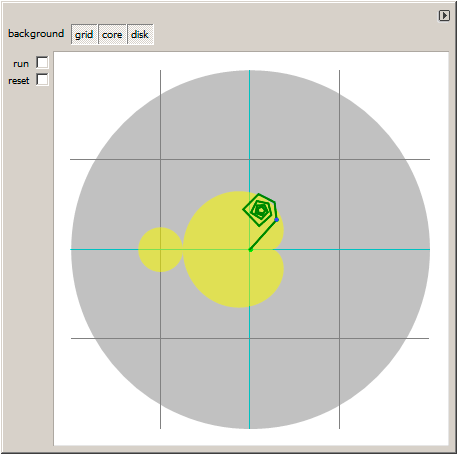
\includegraphics[scale=\FigScale]{examples/demos/mandelbrot/demo1.png}
\caption{\RU{Я кликнул внутри желтой области}\EN{I clicked inside yellow area}}
\end{figure}

\RU{Это значит, что точка на которой я кликнул, находится внутри множества Мандельброта}\EN{This mean, 
the point I clicked belongs to Mandelbrot set}.

\clearpage
\RU{Затем я кликнул снаружи желтой области, и мы видим более хаотичные движения точки, которая быстро выходит
за пределы:}
\EN{Then I clicked outside yellow area and we see much more chaotic point movement, 
which is quickly goes off bounds:}

\begin{figure}[H]
\centering
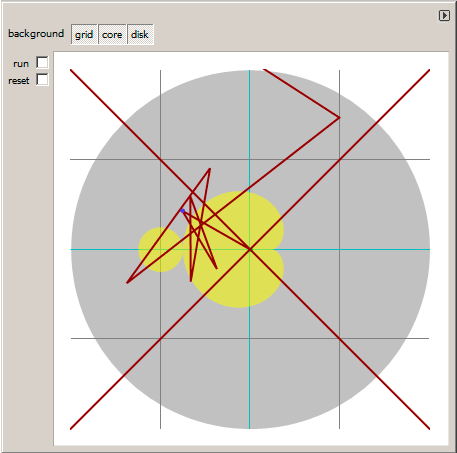
\includegraphics[scale=\FigScale]{examples/demos/mandelbrot/demo2.png}
\caption{\RU{Я кликнул снаружи желтой области}\EN{I clicked outside yellow area}}
\end{figure}

\RU{Это значит, что эта точка не принадлежит множеству Мандельброта}\EN{This mean the point not belongs 
to Mandelbrot set}.

\RU{Другая неплохая демонстрация там}\EN{Another good demo there is}: 
\url{http://go.yurichev.com/17310}.

\clearpage
\subsection{\RU{Вернемся к демо}\EN{Let's back to the demo}}

\RU{Демо, хотя и крошечная (только 64 байта или 30 инструкций), реализует общий алгоритм, изложенный
здесь, но с некоторыми трюками.}
\EN{The demo, although very tiny (just 64 bytes or 30 instructions), implements the common algorithm 
I described here, but using some coding tricks.}

\RU{Исходный код можно скачать, так что вот он, но я также добавил своих комментариев}\EN{Source code is 
easily downloadable, so I got it, but I also added my comments}:

\lstinputlisting[caption=\RU{Исходный код с комментариями}\EN{Commented source code},numbers=left]{examples/demos/mandelbrot/Microbrot_commented.asm.\LANG}

\RU{Алгоритм}\EN{Algorithm}:

\begin{itemize}
\item \RU{Переключаемся в режим VGA}\EN{Switch to} 320*200 \RU{256 цветов}\EN{VGA video mode, 256 colors}. 
$320*200=64000$ (0xFA00). 
\RU{Каждый пиксель кодируется одним байтом, так что размер буфера 0xFA00 байт.}
\EN{Each pixel encoded by one byte, so the buffer size is 0xFA00 bytes.}
\RU{Он адресуется здесь при помощи пары регистров ES:DI}\EN{It is addressed as ES:DI registers pairs}.

\index{x86!\Registers!ES}
ES \RU{должен быть здесь}\EN{should be} 0xA000\RU{, потому что это сегментный адрес видеобуфера, но запись
числа 0xA000 в ES потрубет по крайней мере 4 байта}\EN{ here, because this is segment address of 
VGA video buffer, but storing 0xA000 to ES requires at least 4 bytes} (\TT{PUSH 0A000h / POP ES}). 
\RU{О 16-битной модели памяти в MS-DOS, читайте больше тут}\EN{Read more about 16-bit MS-DOS memory model}: 
\ref{8086_memory_model}.

\index{x86!\Instructions!LES}
\RU{Учитывая, что BX здесь 0, и Program Segment Prefix находится по нулевому адресу, 2-байтная инструкция
\TT{LES AX,[BX]} запишет 0x20CD в AX и 0x9FFF в ES.}
\EN{Assuming, BX is zero here, and Program Segment Prefix is at zeroth
address, 2-byte \TT{LES AX,[BX]} instruction will store 0x20CD to AX and 0x9FFF to ES.}
\RU{Так что программа начнет рисовать на 16 пикселей или байт перед видеобуфером.}
\EN{So, the program will start to draw 16 pixels or bytes before actual video buffer.}
\RU{Но это}\EN{But this is} MS-DOS, \RU{здесь нет защиты памяти, так что ничего плохого не произойдет}\EN{there 
are no memory protection, so nothing will crash}.
\RU{Вот почему вы видите красную полосу шириной 16 пикселей справа}\EN{That's why you see red strip of 16 
pixels width at right}.
\RU{Вся картинка сдвинута налево на 16 пикселей}\EN{Whole picture is shifted left by 16 pixels}.
\RU{Это цена экономии 2-х байт}\EN{This is the price of 2 bytes saving}.

\item \RU{Вечный цикл, обрабатывающий каждый пиксель}\EN{Eternal loop processing each pixel}.
\RU{Наверное, самый общий метод обойти все точки на экране это два цикла:
один для X-координаты, второй для Y-координаты.}
\EN{Probably, most common way to enumerate all pixels on screen is two loops: 
one for X-coordinate, another for Y-coordinate.}
\RU{Но тогда вам придется перемножать координаты для поиска байта в видеобуфере VGA}\EN{But then you'll need 
to multiplicate coordinates to find a byte in VGA video buffer}.
\RU{Автор этого демо решил сделать наоборот: перебирать все байты в видеобуфере при помощи одного цикла
вместо двух и затем получать координаты текущей точки при помощи деления.}
\EN{Author of this demo decide to do it otherwise: enumerate all bytes in video buffer by one single loop instead 
of two, and get coordinates of current point using division.}
\RU{В итоге координаты такие: X в пределах}\EN{Resulting coordinates are: X in range of} $-100..99$ \AndENRU Y 
\RU{в пределах}\EN{in range of} $-256..63$.
\RU{Вы можете увидеть на скриншоте что картинка как бы сдвинута в правую часть экрана}\EN{You may see on 
screenshot that picture is somewhat shifted to the right part of screen}.
\RU{Это потому что самая большая черная дыра в форме сердца обычно появляется на координатах 0,0 и они
здесь сдвинуты вправо.}
\EN{That's because the biggest heart-shaped black hole is usually appears on coordinates 0,0 and these are shifted
here to right.}
\RU{Мог ли автор просто отнять 160 от X, чтобы получилось значение в пределах}\EN{Could author just 
subtract 160 from value to get X in range of} $-160..159$? 
\RU{Да, но инструкция}\EN{Yes, but instruction} \TT{SUB DX, 160} \RU{занимает 4 байта}\EN{takes 4 bytes}, 
\RU{тогда как}\EN{while} \TT{DEC DH}\EMDASH{}2 \RU{байта}\EN{bytes} 
(\RU{которая отнимает}\EN{which subtracts} 0x100 (256) \RU{от}\EN{from} DX). 
\RU{Так что картинка сдвинута ценой экономии еще 2-х байт}\EN{So the whole picture shifted is the cost of 
another 2 bytes of saved space}.

    \begin{itemize}
    \item \RU{Проверить, является ли текущая точка внутри множества Мандельброта}\EN{Check, if the current 
point is inside Mandelbrot set}.
          \RU{Алгоритм такой же, как я описал}\EN{The algorithm is the same I described}.
\index{x86!\Instructions!LOOP}
     \item \RU{Цикл организуется инструкцией \TT{LOOP}, которая использует регистр CX как счетчик}\EN{The loop 
is organized used \TT{LOOP} instructions, which use CX register as counter}.
\RU{Автор мог бы установить число итераций на какое-то число, но не сделал этого: потому что 320 уже
находится в CX (было установлено на строке 35), и это итак подходящее число как число максимальных
итераций.}
\EN{Author could set iteration number to some specific number, but he didn't: 320 is already in CX 
(was set at line 35), and this is good maximal iteration number anyway.}
\RU{Мы здесь экономим немного места, не загружая другое значение в регистр CX}\EN{We save here some space 
by not reloading CX register with other value}.

\index{x86!\Instructions!SAR}
     \item \RU{Здесь используется \TT{IMUL} вместо \TT{MUL}, потому что мы работаем с знаковыми значениями:
помните, что координаты 0,0 должны быть где-то рядом с центром экрана.}
\EN{\TT{IMUL} is used here instead of \TT{MUL}, because we work with signed values: 
remember that 0,0 coordinates should be somewhere near screen center.}
\RU{Тоже самое и с \TT{SAR} (арифметический сдвиг для знаковых значений): она используется вместо \TT{SHR}.}
\EN{The same thing about \TT{SAR} (arithmetic shift for signed values): it's used instead of \TT{SHR}.}

     \item \RU{Еще одна идея --- это упростить проверку пределов}\EN{Another idea is to simplify bounds check}.
\RU{Нам бы пришлось проверять пару координат, т.е., две переменных}\EN{We would need to check coordinate pair, 
i.e., two variables}.
\RU{Что делает автор это трижды проверяет на переполнение: две операции возведения в квадрат и одно 
прибавление}\EN{What author does is just checks thrice for overflow: two square operations and one addition}.
\RU{Действительно, мы ведь используем 16-битные регистры, содержащие знаковые значения в пределах}
\EN{Indeed, we use 16-bit registers, which holds signed values in range of} $-32768..32767$, \RU{так что
если любая из координат больше чем 32767 в процессе умножения, точка однозначно вышла за пределы,
и мы переходим на метку \TT{MandelBreak}.}
\EN{so if any of coordinate is greater than 32767 during signed multiplication, this point is definitely out 
of bounds: we jump to \TT{MandelBreak} label.}

     \item \RU{Здесь также имеется деление на 64 (при помощи инструкции SAR). 64 задает масштаб.}
\EN{There are also division by 64 (SAR instruction). 64 sets scale.}
\RU{Попробуйте увеличить значение и вы получите более увеличенную картинку, или уменьшить для
меньшей.}
\EN{Try to increase value and you will get closer look, or to decrease to more distant look.}

    \end{itemize}

\item \RU{Мы находимся на метке}\EN{We are at} \TT{MandelBreak}\EN{ label}, \RU{есть только две возможности
попасть сюда}\EN{there are two ways of getting here}: 
\RU{цикл закончился с}\EN{loop ended with} CX=0 (\RU{точка внутри множества Мандельброта}
\EN{point is inside Mandelbrot set}); \RU{или потому что произошло переполнение (CX все еще содержит 
какое-то значение)}\EN{or because overflow was happened (CX still holds some value)}.
\RU{Записываем 8-битную часть CX (CL) в видеобуфер}\EN{Now we write low 8-bit part of CX (CL) to the 
video buffer}.
\RU{Палитра по умолчанию грубая, тем не менее, 0 это черный: поэтому видим черные дыры в местах где точки
внутри множества Мандельброта.}
\EN{Default palette is rough, nevertheless, 0 is black: hence we see black holes in places where points are
in Mandelbrot set.}
\RU{Палитру можно инициализировать в начале программы, но не забывайте, это всего лишь программа на 64 
байта}\EN{Palette can be initialized at program start, but remember, that's only 64 bytes program}!

\item \RU{Программа работает в вечном цикле, потому что дополнительная проверка, где остановится, 
или пользовательский интерфейс, это дополнительные инструкции}\EN{Program is running in eternal loop, 
because additional check where to stop, or user interface is additional instructions}.

\end{itemize}

\RU{Еще оптимизационные трюки}\EN{Some other optimization tricks}:

\begin{itemize}
\index{x86!\Instructions!CWD}
\item 1-\RU{байтная}\EN{byte} CWD \RU{используется здесь для обнуления DX вместо двухбайтной}\EN{is used here 
for clearing DX instead of 2-byte} \TT{XOR DX, DX} \RU{или даже трехбайтной}\EN{or even 3-byte} \TT{MOV DX, 0}.

\item 1-\RU{байтная}\EN{byte} \TT{XCHG AX, CX} \RU{используется вместо двухбайтной}\EN{is used instead of 2-byte} 
\TT{MOV AX,CX}. 
\RU{Текущее значение в AX все равно уже не нужно}\EN{Current AX value is not needed here anyway}.

\item DI (\RU{позиция в видеобуфере}\EN{position in video buffer}) \RU{не инициализирована, и будет 0xFFFE в
начале}\EN{is not initialized, and it is 0xFFFE at start}
\footnote{\RU{Больше о состояниях регистров на старте}\EN{More information about initial register values}: 
\url{http://go.yurichev.com/17004}}.
\RU{Это нормально, потому что программа работает бесконечно для всех DI в пределах 0..0xFFFF, и пользователь
не заметит, что работала началась за экраном (последний пиксель видеобуфера 320*200 имеет адрес 0xF9FF).}
\EN{That's OK, because the program works for all DI in range of 0..0xFFFF eternally, and user will not notice
it was started off the screen (last pixel of 320*200 video buffer is at the address 0xF9FF).}
\RU{Так что некоторая часть работы на самом деле происходит за экраном}\EN{So some work is actually done 
off the limits of screen}.
\RU{А иначе понадобятся дополнительные инструкции для установки DI в 0; добавить проверку на конец буфера.}
\EN{Otherwise, you'll need additional instructions to set DI to 0; check for video buffer end.}

\end{itemize}

\newcommand{\MyFixedVersion}{\RU{Моя ``исправленная'' версия}\EN{My ``fixed'' version}}
\subsection{\MyFixedVersion}

\lstinputlisting[caption=\MyFixedVersion,numbers=left]{examples/demos/mandelbrot/my_version.asm.\LANG}

\RU{Я попытался исправить все эти странности: теперь палитра плавная черно-белая, видеобуфер на правильном месте
(строки 19..20), картинка рисуется в центре экрана (строка 30), программа в итоге заканчивается и ждет,
пока пользователь нажмет какую-нибудь клавишу (строки 58..68).}
\EN{I made attempt to fix all these oddities: now palette is smooth grayscale, video buffer is at correct place 
(lines 19..20),
picture is drawing on center of screen (line 30), program eventually ends and waiting for user keypress 
(lines 58..68).}
\RU{Но теперь она намного больше: 105 байт (или 54 инструкции)}
\EN{But now it's much bigger: 105 bytes (or 54 instructions)}
\footnote{\RU{Можете поэкспериментировать и сами: скачайте DosBox и NASM и компилируйте так:}
\EN{You can experiment by yourself: get DosBox and NASM and compile it as:} 
\TT{nasm fiole.asm -fbin -o file.com}}.

\begin{figure}[H]
\centering
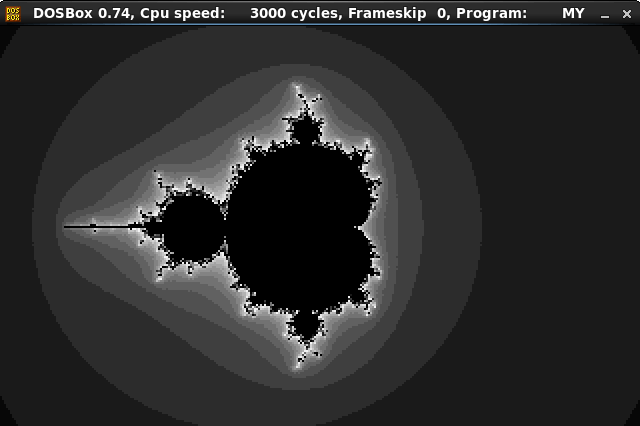
\includegraphics[scale=\FigScale]{examples/demos/mandelbrot/fixed.png}
\caption{\MyFixedVersion}
\label{fig:mandelbrot_fixed}
\end{figure}
